% id: 52-13
% book: 개념원리 중학 3-2 · 05 넓이 구하기
% section: 중단원 마무리하기 STEP 2 발전 문제
% figure: crop:fig-52-13.png
% answer: ④
% answer_source: 답지
% variant_level: 0 (원본 전사)
% 이 파일은 build.mjs 가 items.json 에서 만든다. 고칠 때는 items.json 을 고친다.
\smash{\raisebox{1.5mm}{\dmkichul{개념원리 중학 3-2 52쪽 13번}}}
\noindent\begin{minipage}[t]{0.58\linewidth}\vspace{0pt}\raggedright 오른쪽 그림과 같이 길이가 $40\mkern3mu \mathrm{cm}$인 실에 매달린 추가 $\seg{OA}$를 기준으로 좌우로 $30^\circ$의 각을 이루며 움직이고 있다. 이때 지점~$\pt{B}$는 지점~$\pt{A}$보다 몇 $\mathrm{cm}$ 더 높은가? \cond{추의 크기는 생각하지 않는다.}\end{minipage}\hfill\begin{minipage}[t]{0.4\linewidth}\vspace{0pt}\centering \setlength{\dmfigw}{67.2pt}\ifdim\dmfigw>\linewidth\setlength{\dmfigw}{\linewidth}\fi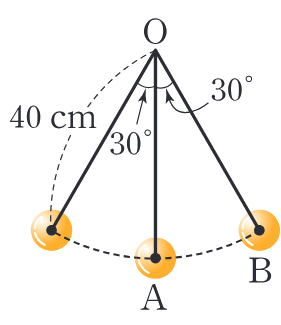
\includegraphics[width=\dmfigw]{figures/fig-52-13.png}\end{minipage}\par
\begin{choicesii}{\rule[-3ex]{0pt}{8ex}$(20-10\sqrt{3})\mkern3mu \mathrm{cm}$}{\rule[-3ex]{0pt}{8ex}$3\mkern3mu \mathrm{cm}$}{\rule[-3ex]{0pt}{8ex}$5\mkern3mu \mathrm{cm}$}{\rule[-3ex]{0pt}{8ex}$(40-20\sqrt{3})\mkern3mu \mathrm{cm}$}{\rule[-3ex]{0pt}{8ex}$(10\sqrt{3}-10)\mkern3mu \mathrm{cm}$}\end{choicesii}
